\chapter{SatNOGS: Глобальная сеть наземных спутниковых станций с открытым исходным кодом}

SatNOGS представляет собой комплексную платформу \cite{satnogs_general_docs},
обеспечивающую функционирование открытой сети наземных станций для мониторинга
спутников. Основной целью проекта является разработка полного стека открытых
технологий, основанных на открытых стандартах, и создание полноценной наземной
станции в качестве демонстрации возможностей данного стека.

Система SatNOGS способна принимать сигналы со спутников, находящихся на низкой
околоземной орбите (LEO), в диапазонах UHF и VHF. Она позволяет извлекать
сигналы состояния и телеметрии, данные с научных и исследовательских спутников
(например, результаты магнитосферных экспериментов), метеорологические данные и
другую информацию.

Проект SatNOGS включает в себя несколько ключевых компонентов: веб-приложение
для планирования наблюдений, базу данных для хранения информации о спутниках,
клиентское программное обеспечение для работы на наземных станциях и аппаратное
обеспечение с открытым исходным кодом. Все это создает модульную архитектуру,
позволяющую легко интегрировать новые функции и расширять функциональность
системы.

SatNOGS активно развивает сообщество пользователей и разработчиков, предлагая
доступ к документации и инструментам для создания собственных наземных станций.
Это создает возможности для участия в глобальной сети наблюдений за спутниками
и обмена данными между участниками проекта.

\section{Компоненты SatNOGS}

SatNOGS включает в себя несколько ключевых компонентов, каждый из которых
играет важную роль в функционировании платформы, см. рисунок
\ref{fig:satnogs_data_flow}.
Ниже представлена таблица, описывающая основные элементы системы:

\begin{table}[h]
	\centering
	\begin{tabular}{|l|p{10cm}|}
		\hline \textbf{Компонент} & \textbf{Описание}
		\\ \hline SatNOGS Network          & Веб-приложение, предназначенное для
		планирования наблюдений по сети наземных станций. Оно способствует
		координации наблюдений за спутниковыми сигналами и планированию таких
		наблюдений среди наземных станций, подключенных к сети.                                 \\ \hline База
		данных SatNOGS            & Ресурс, позволяющий пользователям предоставлять
		информацию о передатчиках активных спутников. Данные доступны через API или
		веб-интерфейс.
		\\ \hline Клиент SatNOGS           & Программное обеспечение, работающее на
		наземных станциях (обычно на встраиваемых системах). Оно получает
		регулярные задания на наблюдение из сети, принимает спутниковые передачи и
		отправляет их обратно в веб-приложение Network.                                         \\ \hline Наземная станция
		SatNOGS                   & Аппаратное обеспечение наземной станции с открытым исходным
		кодом, включающее ротаторы, антенны и электронику, подключенные к клиенту.
		\\ \hline SatNOGS Dashboard        & Веб-интерфейс для визуализации и
		анализа данных телеметрии, полученных от спутников. Он предоставляет
		пользователям возможность отслеживать состояние спутников и их сигналы в
		реальном времени.                                                                       \\ \hline
	\end{tabular}
	\caption{Основные компоненты системы SatNOGS}
	\label{tab:satnogs_components}
\end{table}

Система SatNOGS активно развивает сообщество пользователей и разработчиков,
предлагая доступ к документации и инструментам для создания собственных
наземных станций. Это создает возможности для участия в глобальной сети
наблюдений за спутниками и обмена данными между участниками проекта.

\begin{figure}[htbp]
	\centering
	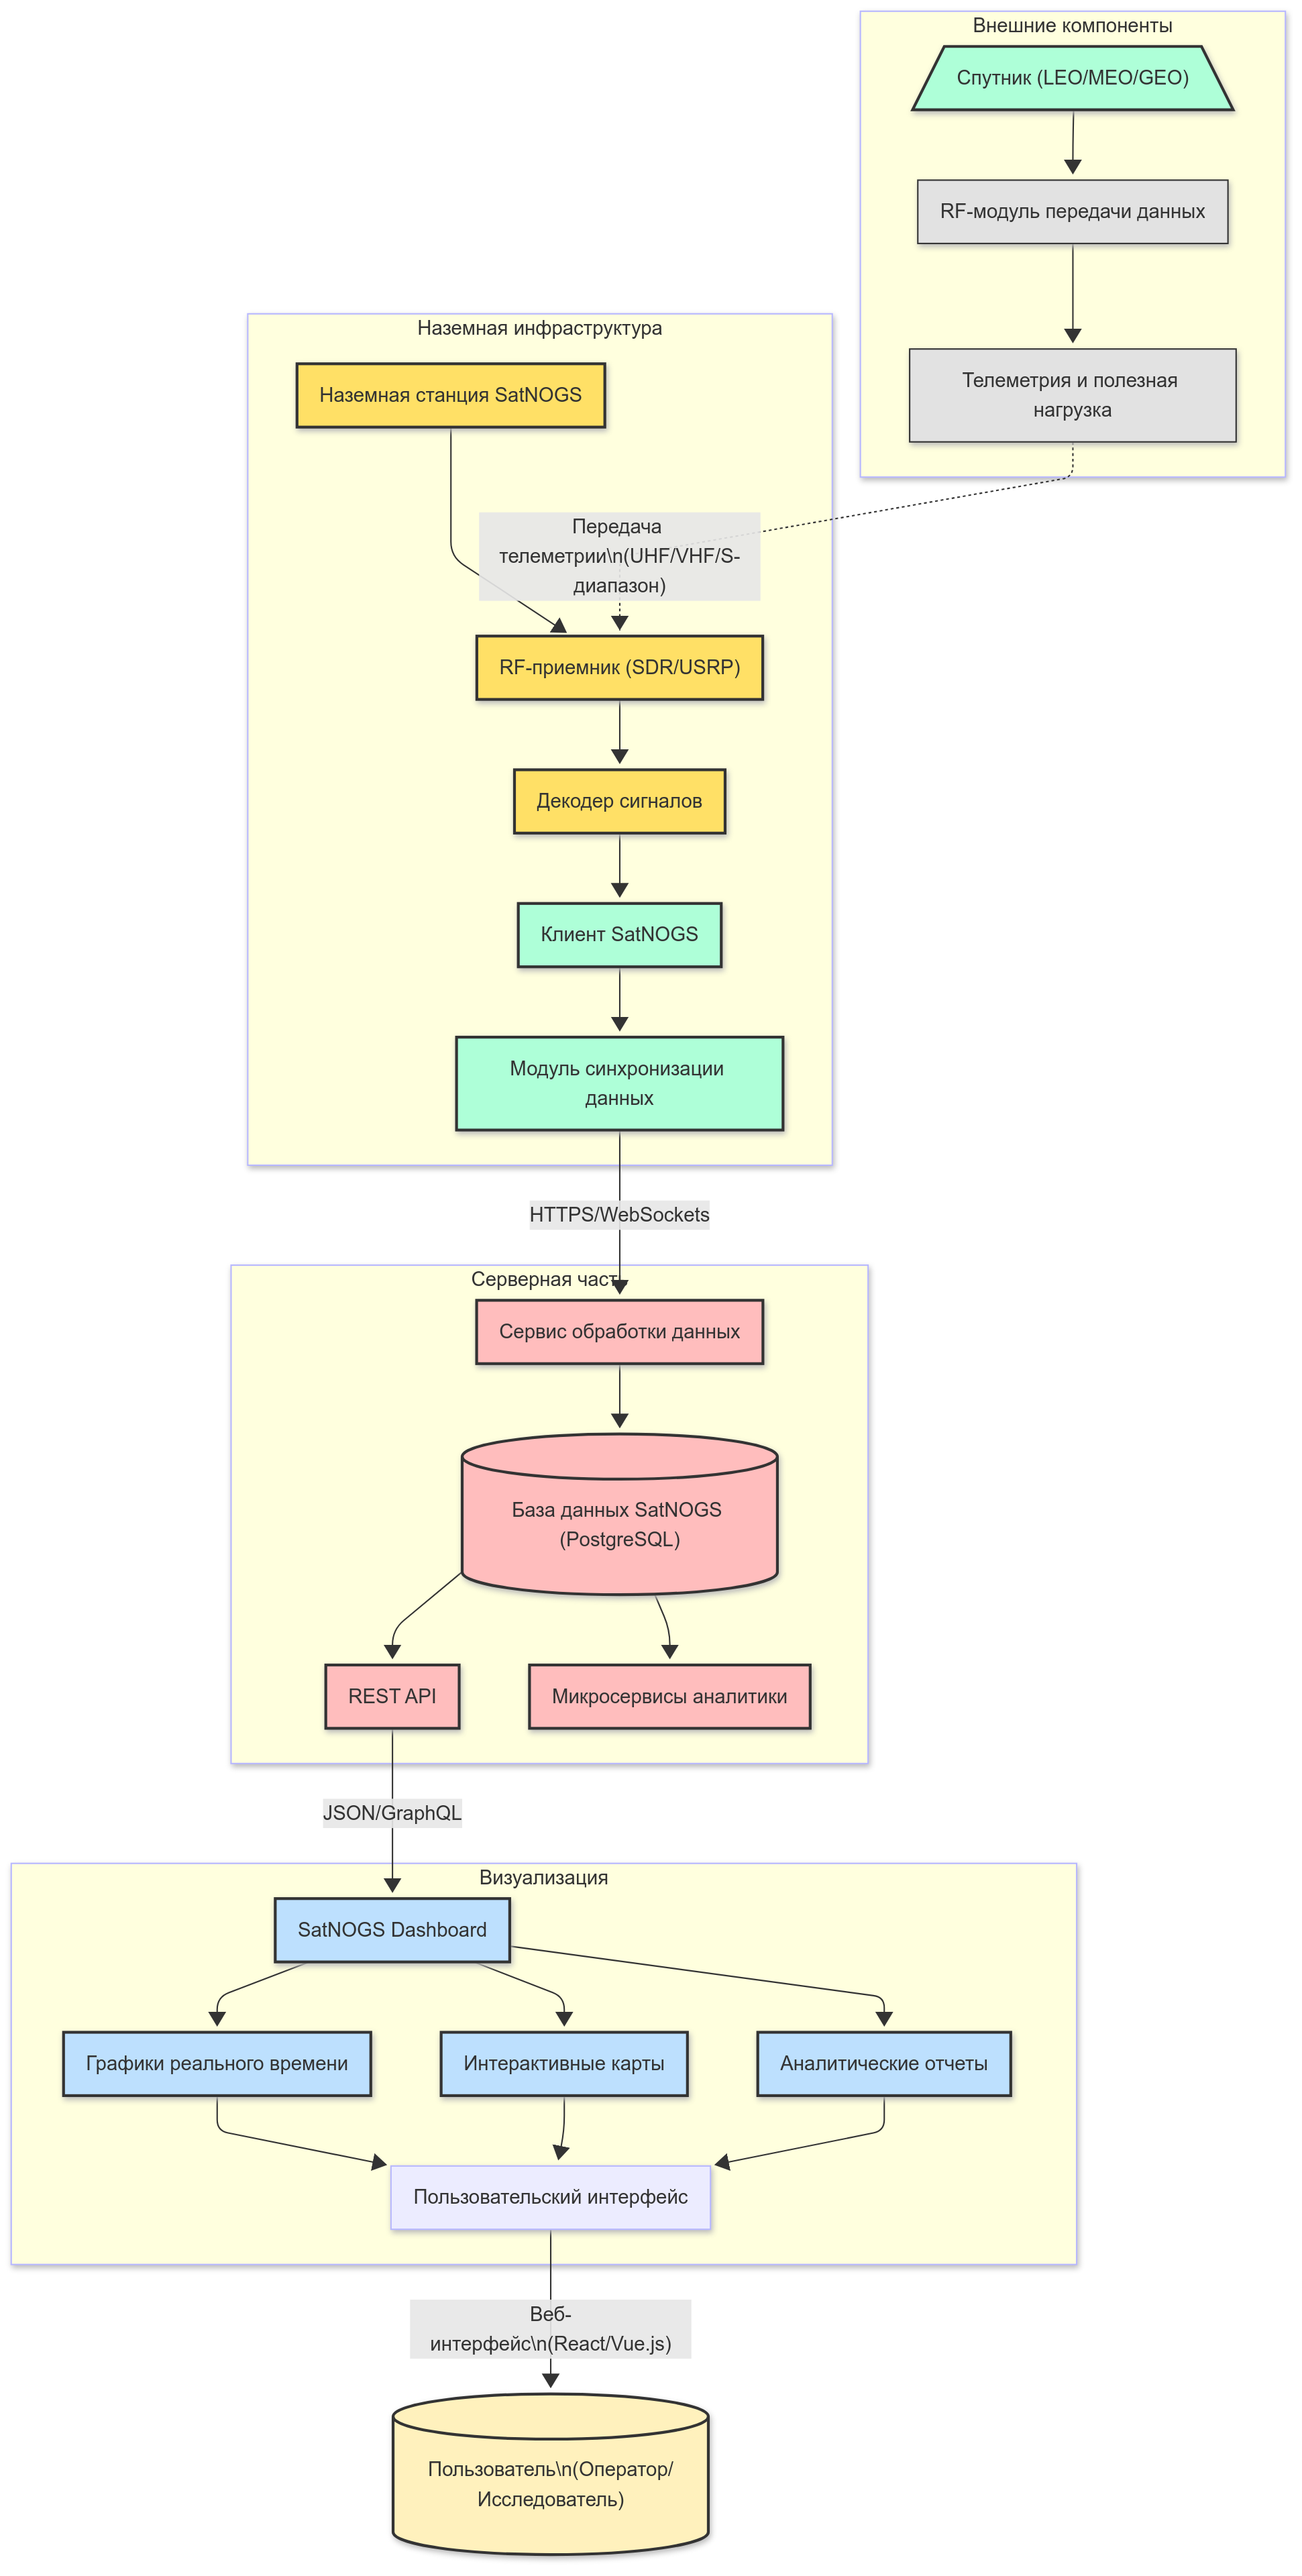
\includegraphics[width=0.7\textwidth]{satnogs_data_flow}
	\caption{Поток данных SatNOGS в Dashboard endpoint}
	\label{fig:satnogs_data_flow}
\end{figure}

\section{SatNOGS Dashboard}

\begin{figure}[htbp]
	\centering
	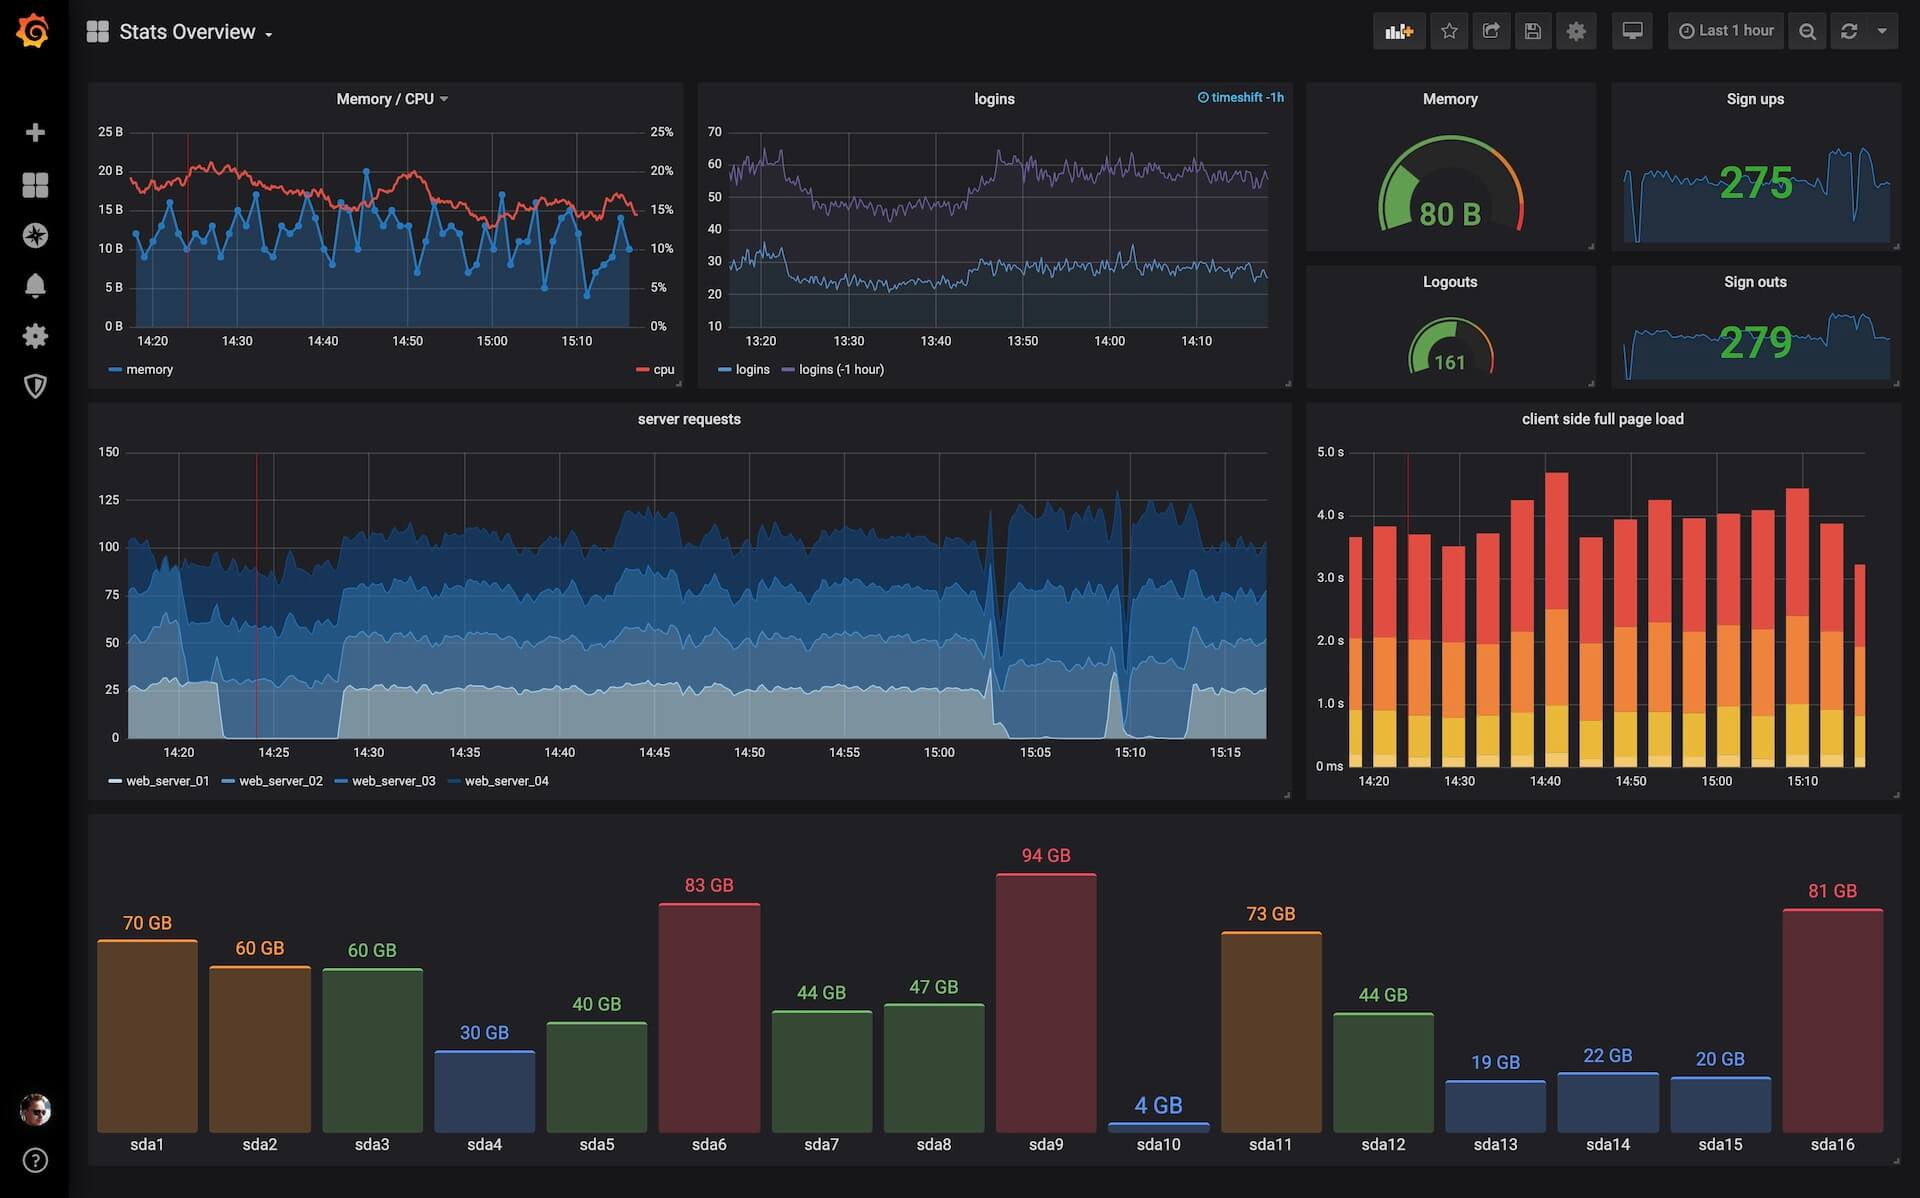
\includegraphics[width=1.0\textwidth]{grafana_example}
	\caption{Пример страницы с данными в Grafana Enterprise}
	\label{fig:grafana_example}
\end{figure}

Основная задача системы SatNOGS Dashboard для нас — получение данных для
обучения. Изучив структуру мы можем выбрать наиболее удобное место для
получения(скрапинга) данных. Наиболее удобным местом оказывается satnogs
dashboard, как ранее говорилось и показывалось на схемах туда закидываются уже
готовые данные, профильтрованные и избавленные от дубликатов путем построения
временного ряда dashboard grafana. Из минусов - неполный перечень спутников,
порядка 120 спутников имеют свои представления. Но этого количества данных нам
уже достаточно, чтобы проанализировать критические метрики и сэкономить время и
ресуры на обучение, отвязавшись от инфраструктуры satnogs.


Grafana — это мощная платформа для визуализации и анализа данных, которая
позволяет создавать интерактивные дашборды на основе различных источников
данных \cite{grafana_docs}. Пример такого дашборда можно увидеть на рисунке
\ref{fig:grafana_example}.
Grafana широко используется для мониторинга систем и приложений, предоставляя
пользователям возможность отслеживать ключевые метрики в реальном времени.

В контексте SatNOGS Dashboard, Grafana работает с базой данных
\textbf{InfluxDB} \cite{influxdb_docs}, которая предназначена для хранения
временных рядов данных, таких как телеметрия спутников. Данные поступают от
наземных станций, обрабатываются клиентом SatNOGS и сохраняются в InfluxDB.
Затем Grafana использует API для доступа к этим данным и их визуализации на
дашбордах.

Однако стоит отметить, что доступ к API Grafana Dashboard SatNOGS был закрыт,
что ограничивает возможности пользователей в получении данных напрямую. Более
того, Grafana не предоставляет свои услуги пользователям из России и Беларуси в
связи с санциями \cite{grafana_community_post}, что создает дополнительные
сложности для разработчиков и исследователей из этих стран. Это делает Grafana
ненадежной платформой для работы в нашем регионе.

В связи с этими ограничениями нам приходится разрабатывать собственный парсер
для обхода существующих ограничений и получения необходимых данных. Этот парсер
будет рассмотрен далее в нашей работе, так как он позволит нам интегрировать
данные из SatNOGS Dashboard в нашу систему анализа и визуализации.

Таким образом, несмотря на мощные возможности Grafana, текущие ограничения
доступа делают еe менее привлекательной для пользователей из определeнных
регионов, что требует разработки альтернативных решений для работы с данными.
Схему работы SatNOGS Dashboard можно наблюдать на рисунке
\ref{fig:grafana_infra}.

\begin{figure}[htbp]
	\centering
	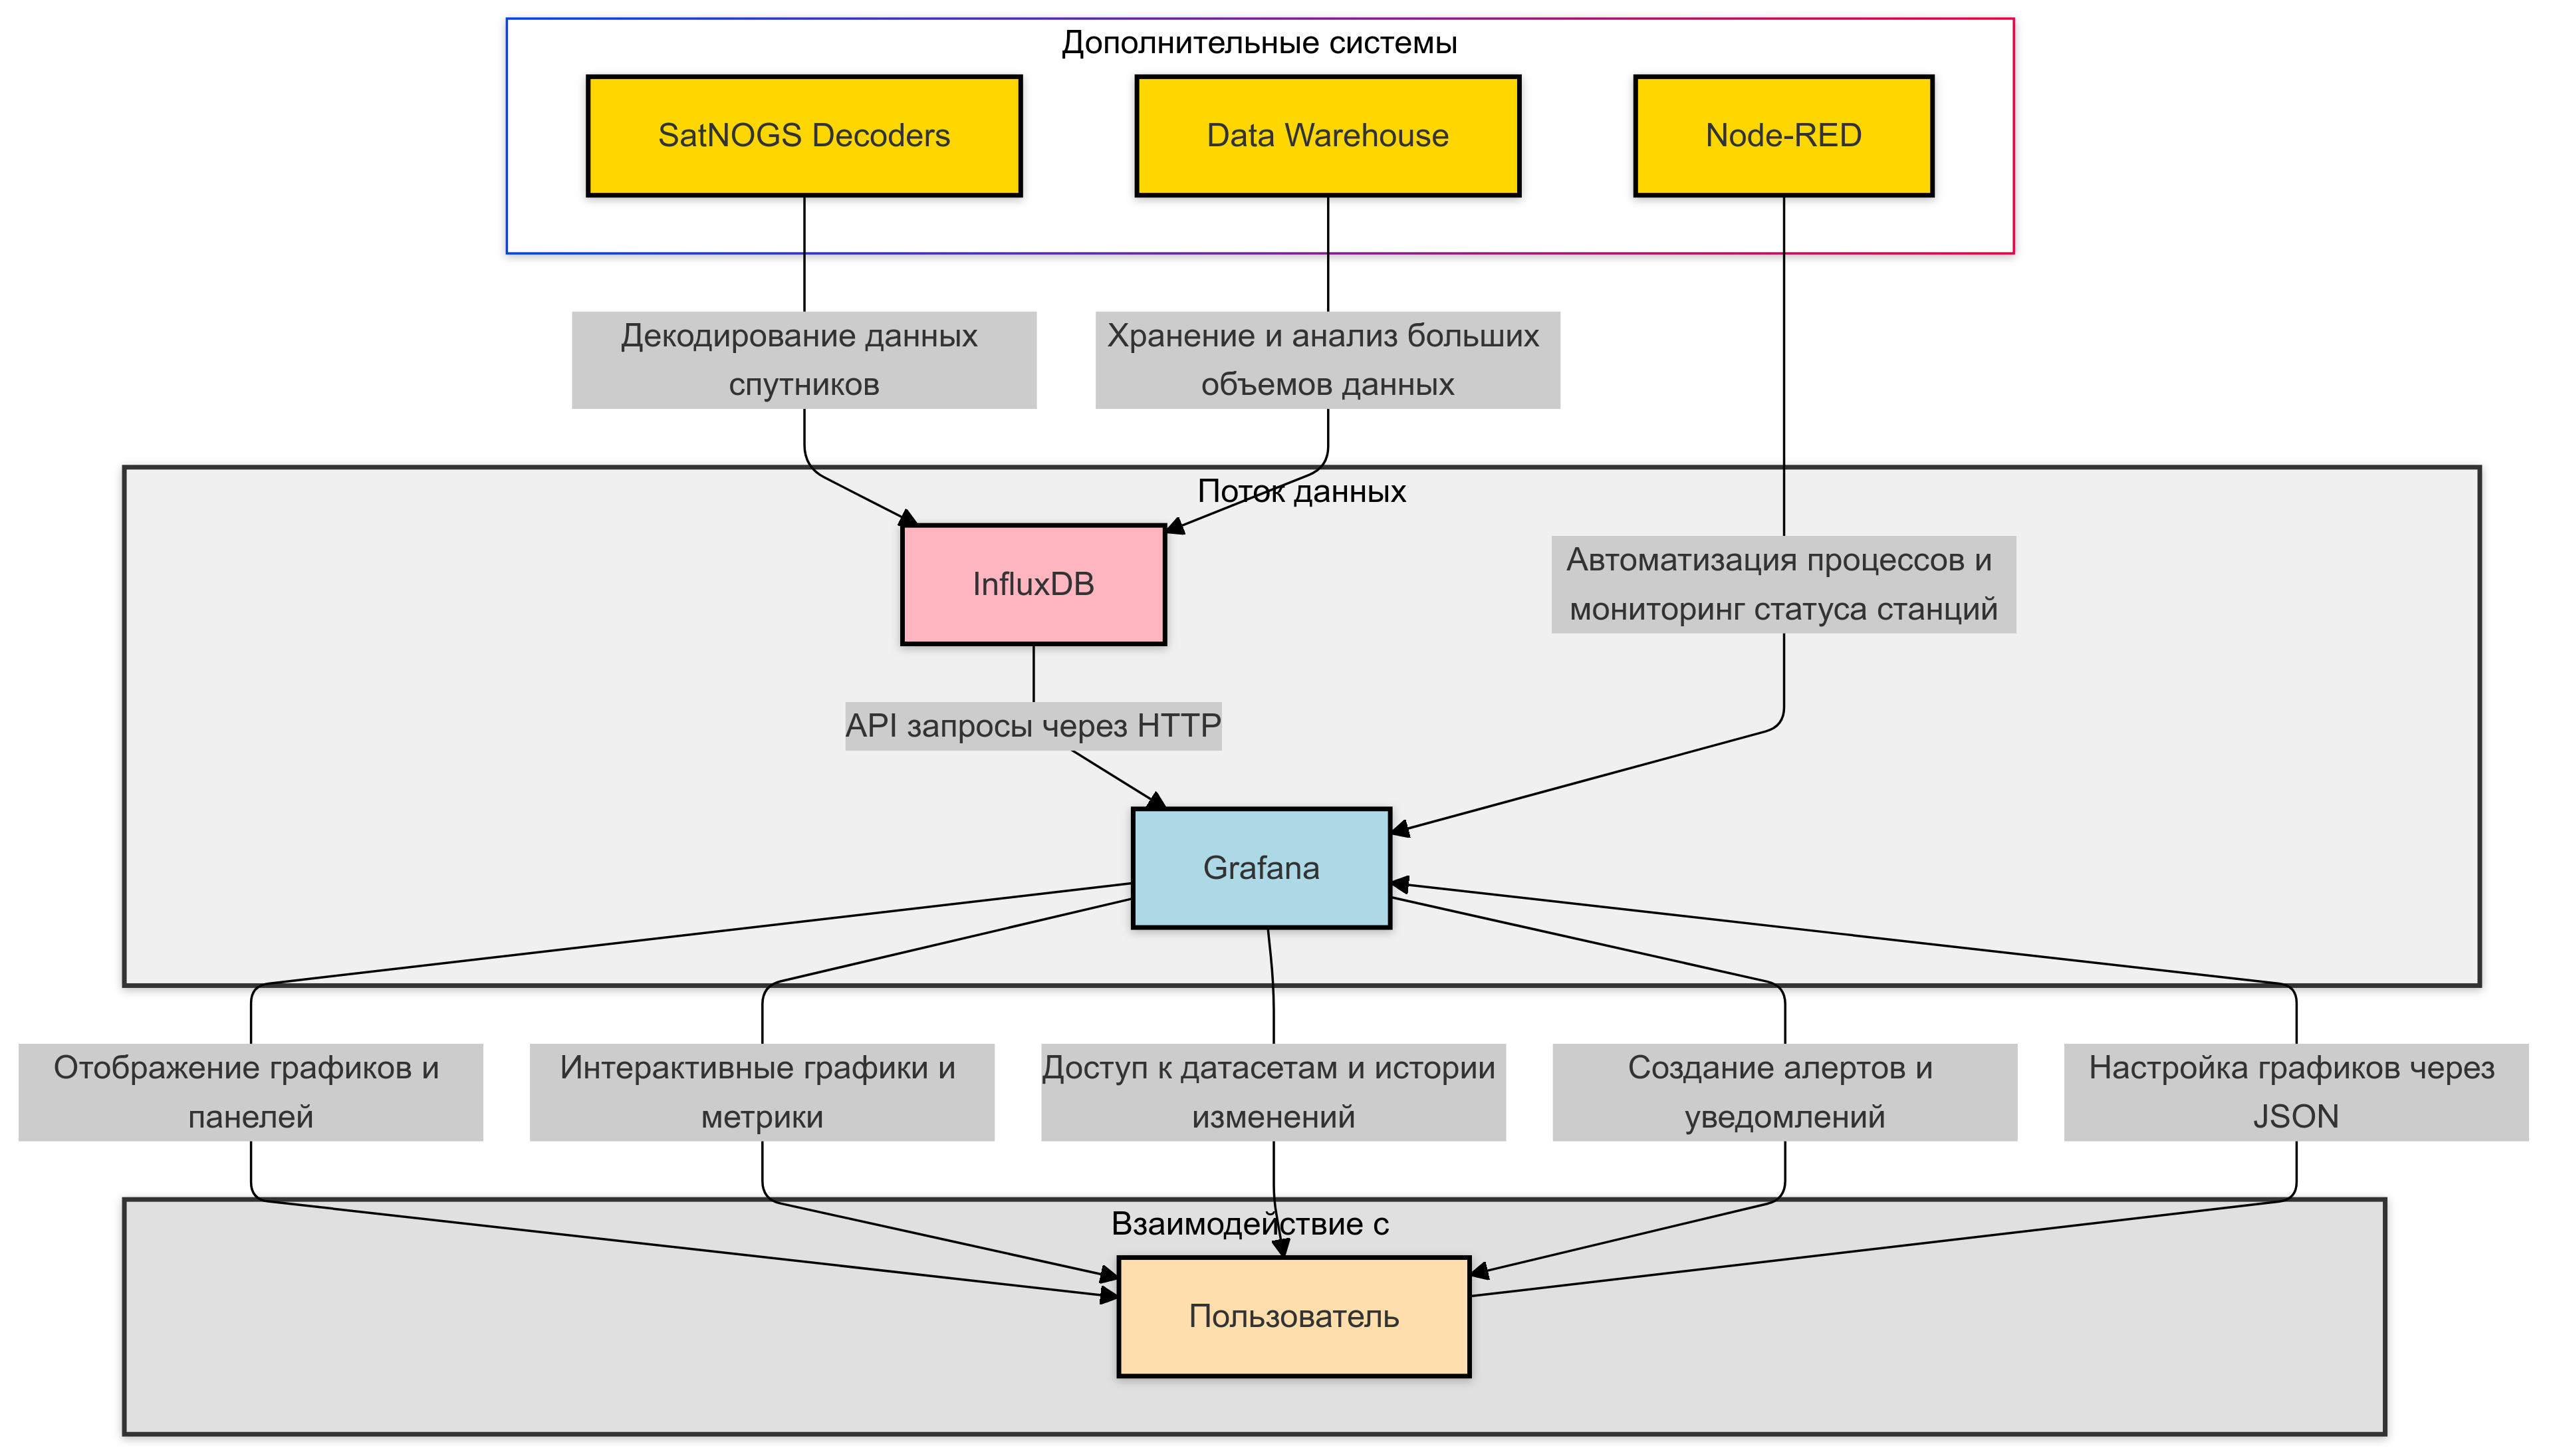
\includegraphics[width=1.0\textwidth]{grafana_infra}
	\caption{Подробное устройство SatNOGS Dashboard}
	\label{fig:grafana_infra}
\end{figure}

\section{Парсинг SatNOGS Dashboard}
\begin{figure}[htbp]
	\centering
	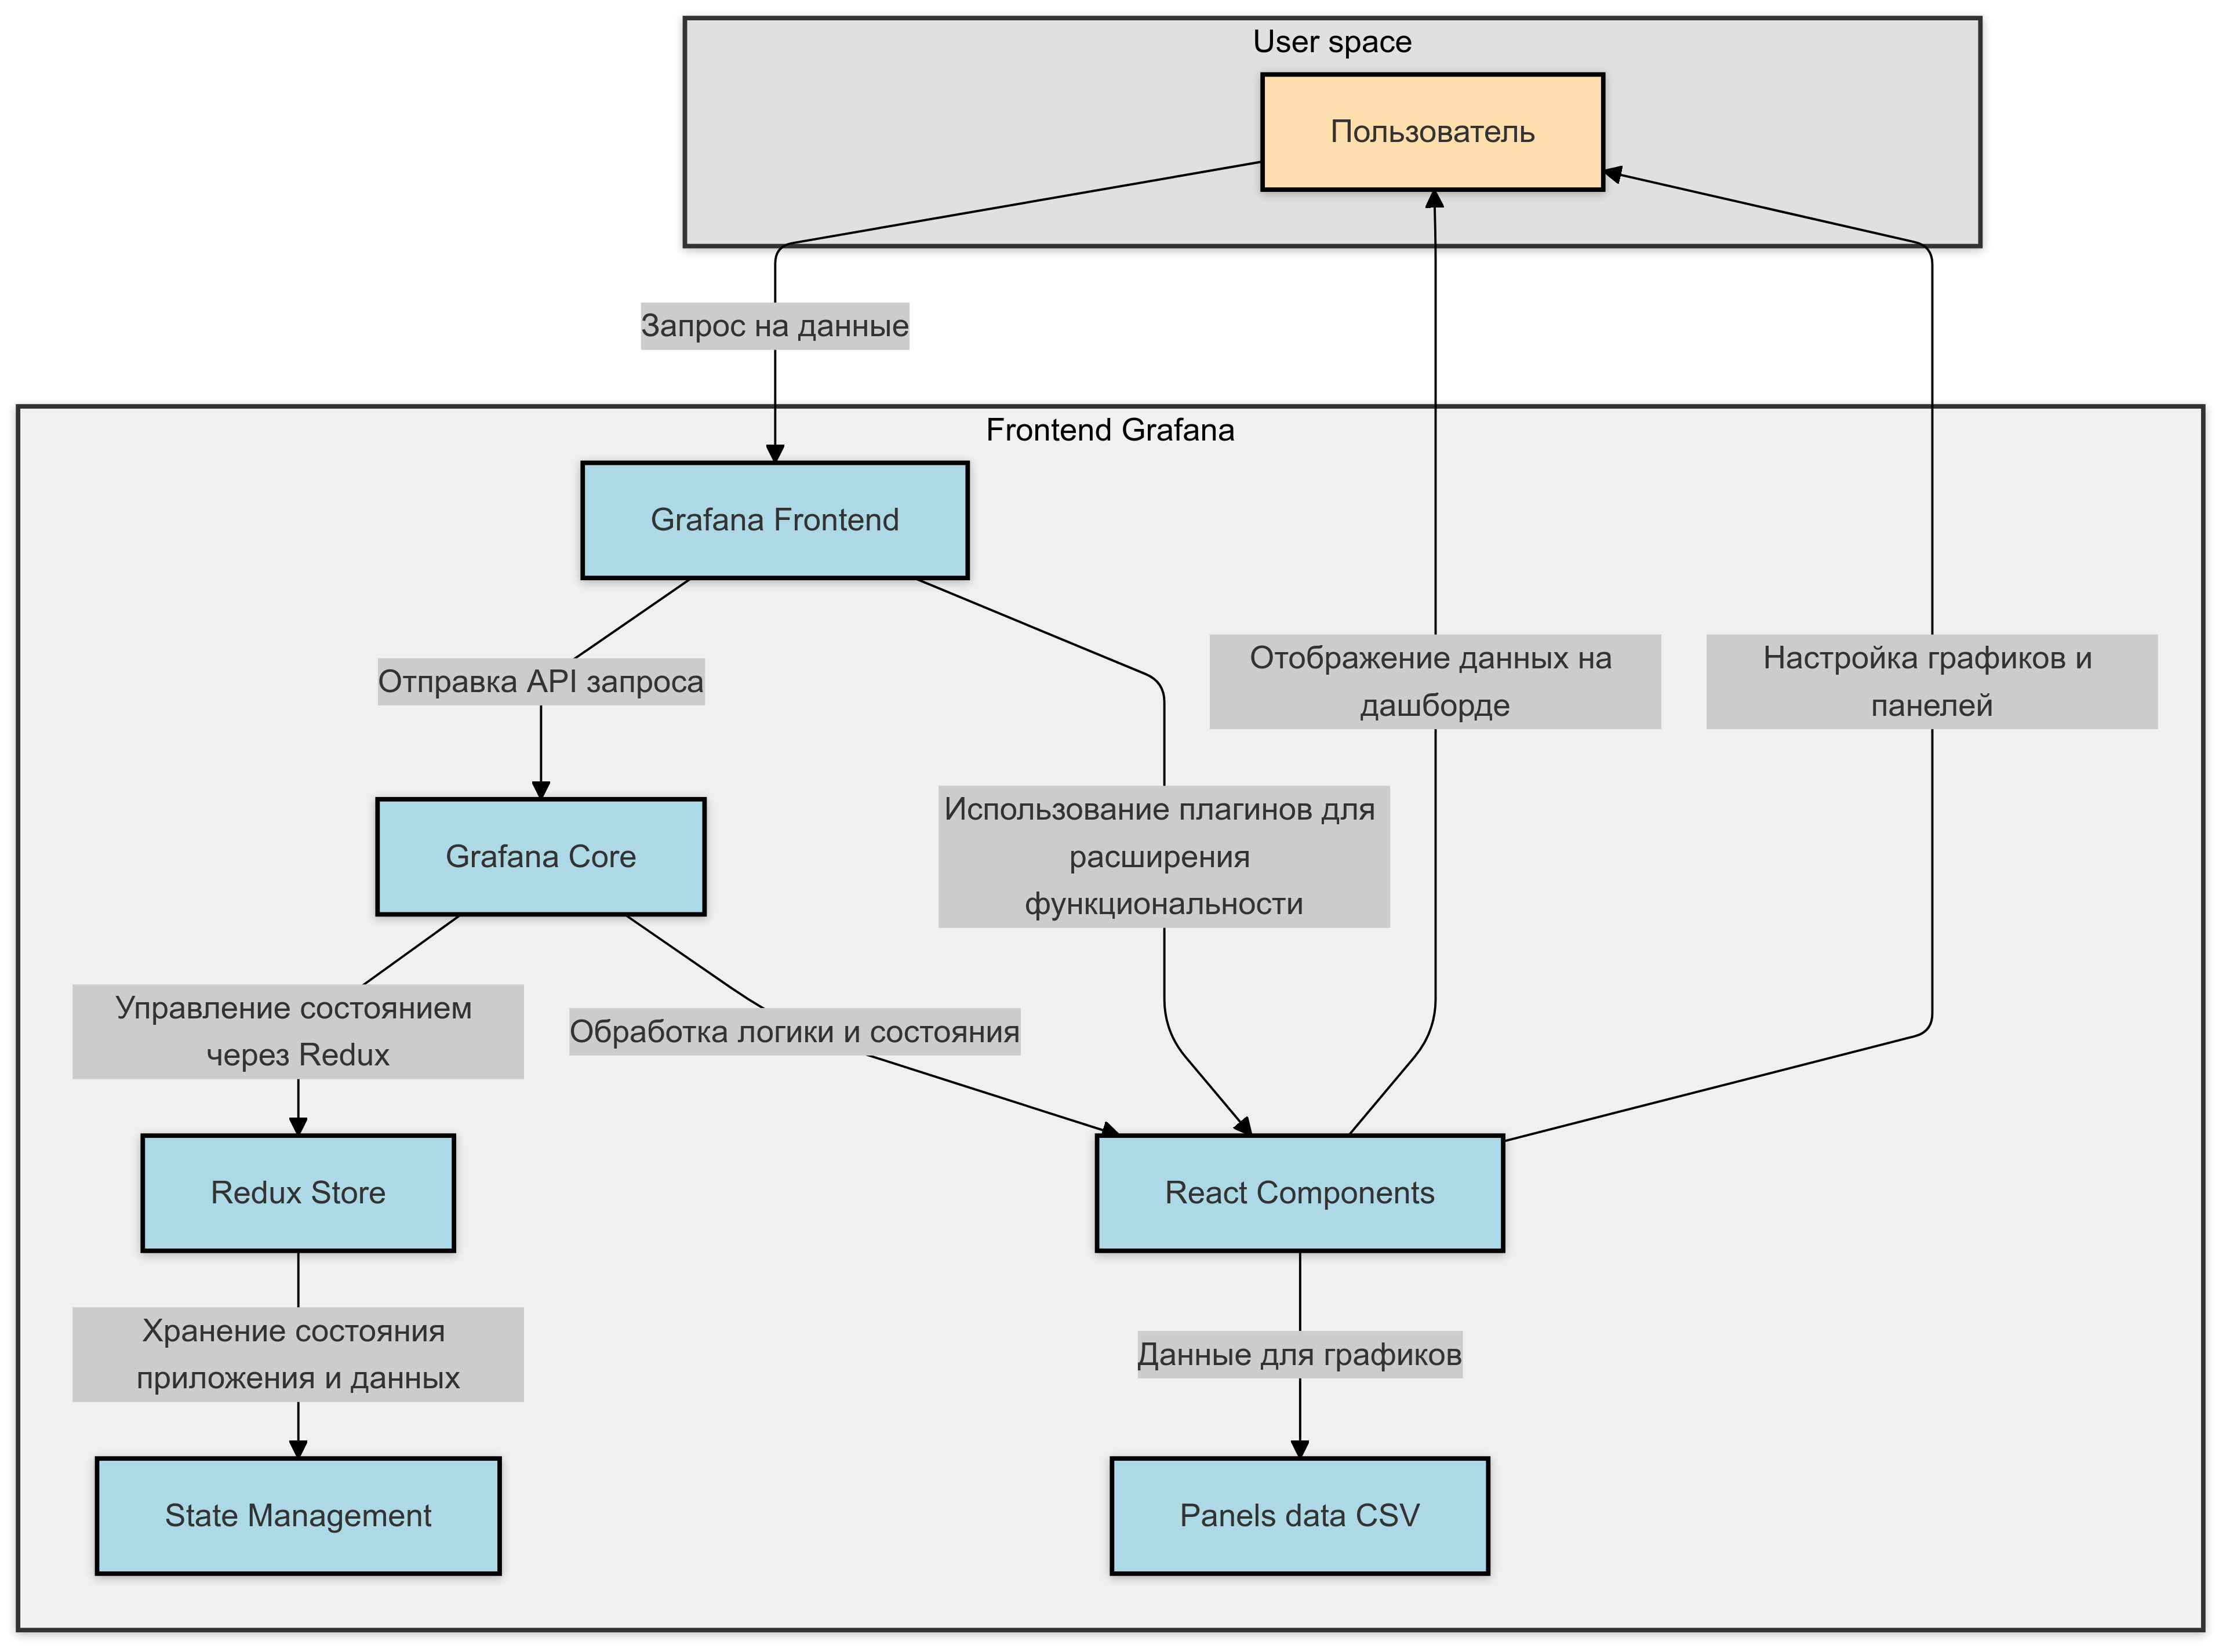
\includegraphics[width=1.0\textwidth]{grafana_frontend_structure}
	\caption{Построение frontend части grafana \cite{react_managing_state}}
	\label{fig:grafana_frontend_structure}
\end{figure}

В рамках нашего проекта по анализу данных спутников мы столкнулись с
необходимостью работы с SatNOGS Dashboard. Это веб-интерфейс, который
предоставляет доступ к данным о спутниках и их телеметрии. Однако, поскольку
API для этого интерфейса является приватным, мы вынуждены прибегать к парсингу
фронтенда с использованием JavaScript, см. рисунок
\ref{fig:grafana_frontend_structure}.

Для начала, мы используем JavaScript для извлечения необходимых данных из
DOM-структуры страницы. Это позволяет нам взаимодействовать с элементами
интерфейса и получать информацию, которая в противном случае была бы
недоступна. Мы реализуем асинхронные функции для ожидания появления элементов
на странице и их обработки.

После того как данные извлечены с помощью JavaScript, мы запускаем скрипт на
Python с использованием библиотеки Selenium WebDriver \cite{selenium_docs}.
Этот подход позволяет автоматизировать взаимодействие с веб-интерфейсом SatNOGS
в нужный момент времени.

Что касается инфраструктуры, мы используем Grafana для визуализации данных.
Grafana интегрируется с различными источниками данных и позволяет создавать
настраиваемые дашборды для мониторинга состояния спутников и анализа
телеметрии. API Grafana предоставляет возможности для динамического обновления
графиков и управления панелями.

Таким образом, мы не только извлекаем данные из SatNOGS Dashboard, но и
используем мощную инфраструктуру для их анализа и визуализации.

\section{Скраппинг данных из SatNOGS dashboard}

Скрипт, написанный на Python с использованием библиотеки Selenium, предназначен
для автоматизации процесса извлечения данных из дашборда Grafana. Он начинается
с настройки логирования и создания веб-драйвера для браузера Firefox с
необходимыми параметрами, такими как директория для загрузки файлов и типы
файлов, которые могут загружаться без подтверждения.

После инициализации драйвера скрипт переходит к идентификации панелей на
дашборде. Он перебирает идентификаторы панелей и проверяет наличие элементов с
соответствующими идентификаторами. Если элемент найден, его заголовок
добавляется в список доступных панелей.

Далее скрипт формирует полный URL для доступа к дашборду с учетом временных
параметров. После загрузки страницы он получает список панелей и создает новый
URL для каждой панели с параметром инспекции. Скрипт ожидает появления
необходимых элементов на странице и инициирует процесс загрузки данных через
выполнение вышеописанного JavaScript-кода.

В заключение, основной блок скрипта определяет список URL-адресов дашбордов,
откуда необходимо загружать данные, и создает директорию для сохранения
загружаемых файлов. В результате работы данного скрипта происходит
автоматическая загрузка данных из Grafana, что значительно упрощает процесс
извлечения информации для дальнейшего анализа или хранения.
